\section{Teilversuch 4: Änderung von lasersicherheitsrelevanten Parametern durch verschiedene optische Instrumente}
	\setcounter{subsection}{2}
	\resnum
	\subsection{Strahlprofil}
		Da ich die Aufgabe 1 in der Vorbereitung falsch gemacht habe, sind die Rechnung hier nachbessert. Mit WolframAlpha erhalten wir:
		\begin{align}
			P = \int_{A} I~\dd A 
			&= \int_{0}^{2\pi} \dd\varphi \int_{0}^{R} \dd r ~ r I_0 \exp{-2\left(\frac{r}{\omega}\right)^2} \notag \\
			&= 2\pi I_0 \int_{0}^{R} \dd r ~ r\exp{-2\left(\frac{r}{\omega}\right)^2} \notag \\
			&= 2\pi I_0 \omega^2 \left[1 - \exp{-2\left(\frac{R}{\omega}\right)^2}\right] \notag
		\end{align}
		Die resultierende Kurve sieht aber genauso aus, wie in der Vorbereitung. Wähle $\omega = \sqrt{2}$ und $I_0 = \frac{1}{4\pi}$ und plotte $1 - \exp{-R^2}$:
		\begin{figure}[H]
			\centering
			% GNUPLOT: LaTeX picture with Postscript
\begingroup
  \makeatletter
  \providecommand\color[2][]{%
    \GenericError{(gnuplot) \space\space\space\@spaces}{%
      Package color not loaded in conjunction with
      terminal option `colourtext'%
    }{See the gnuplot documentation for explanation.%
    }{Either use 'blacktext' in gnuplot or load the package
      color.sty in LaTeX.}%
    \renewcommand\color[2][]{}%
  }%
  \providecommand\includegraphics[2][]{%
    \GenericError{(gnuplot) \space\space\space\@spaces}{%
      Package graphicx or graphics not loaded%
    }{See the gnuplot documentation for explanation.%
    }{The gnuplot epslatex terminal needs graphicx.sty or graphics.sty.}%
    \renewcommand\includegraphics[2][]{}%
  }%
  \providecommand\rotatebox[2]{#2}%
  \@ifundefined{ifGPcolor}{%
    \newif\ifGPcolor
    \GPcolortrue
  }{}%
  \@ifundefined{ifGPblacktext}{%
    \newif\ifGPblacktext
    \GPblacktexttrue
  }{}%
  % define a \g@addto@macro without @ in the name:
  \let\gplgaddtomacro\g@addto@macro
  % define empty templates for all commands taking text:
  \gdef\gplbacktext{}%
  \gdef\gplfronttext{}%
  \makeatother
  \ifGPblacktext
    % no textcolor at all
    \def\colorrgb#1{}%
    \def\colorgray#1{}%
  \else
    % gray or color?
    \ifGPcolor
      \def\colorrgb#1{\color[rgb]{#1}}%
      \def\colorgray#1{\color[gray]{#1}}%
      \expandafter\def\csname LTw\endcsname{\color{white}}%
      \expandafter\def\csname LTb\endcsname{\color{black}}%
      \expandafter\def\csname LTa\endcsname{\color{black}}%
      \expandafter\def\csname LT0\endcsname{\color[rgb]{1,0,0}}%
      \expandafter\def\csname LT1\endcsname{\color[rgb]{0,1,0}}%
      \expandafter\def\csname LT2\endcsname{\color[rgb]{0,0,1}}%
      \expandafter\def\csname LT3\endcsname{\color[rgb]{1,0,1}}%
      \expandafter\def\csname LT4\endcsname{\color[rgb]{0,1,1}}%
      \expandafter\def\csname LT5\endcsname{\color[rgb]{1,1,0}}%
      \expandafter\def\csname LT6\endcsname{\color[rgb]{0,0,0}}%
      \expandafter\def\csname LT7\endcsname{\color[rgb]{1,0.3,0}}%
      \expandafter\def\csname LT8\endcsname{\color[rgb]{0.5,0.5,0.5}}%
    \else
      % gray
      \def\colorrgb#1{\color{black}}%
      \def\colorgray#1{\color[gray]{#1}}%
      \expandafter\def\csname LTw\endcsname{\color{white}}%
      \expandafter\def\csname LTb\endcsname{\color{black}}%
      \expandafter\def\csname LTa\endcsname{\color{black}}%
      \expandafter\def\csname LT0\endcsname{\color{black}}%
      \expandafter\def\csname LT1\endcsname{\color{black}}%
      \expandafter\def\csname LT2\endcsname{\color{black}}%
      \expandafter\def\csname LT3\endcsname{\color{black}}%
      \expandafter\def\csname LT4\endcsname{\color{black}}%
      \expandafter\def\csname LT5\endcsname{\color{black}}%
      \expandafter\def\csname LT6\endcsname{\color{black}}%
      \expandafter\def\csname LT7\endcsname{\color{black}}%
      \expandafter\def\csname LT8\endcsname{\color{black}}%
    \fi
  \fi
    \setlength{\unitlength}{0.0500bp}%
    \ifx\gptboxheight\undefined%
      \newlength{\gptboxheight}%
      \newlength{\gptboxwidth}%
      \newsavebox{\gptboxtext}%
    \fi%
    \setlength{\fboxrule}{0.5pt}%
    \setlength{\fboxsep}{1pt}%
\begin{picture}(8640.00,5760.00)%
    \gplgaddtomacro\gplbacktext{%
      \csname LTb\endcsname%%
      \put(814,704){\makebox(0,0)[r]{\strut{}$0$}}%
      \put(814,1144){\makebox(0,0)[r]{\strut{}$0,1$}}%
      \put(814,1583){\makebox(0,0)[r]{\strut{}$0,2$}}%
      \put(814,2023){\makebox(0,0)[r]{\strut{}$0,3$}}%
      \put(814,2462){\makebox(0,0)[r]{\strut{}$0,4$}}%
      \put(814,2902){\makebox(0,0)[r]{\strut{}$0,5$}}%
      \put(814,3341){\makebox(0,0)[r]{\strut{}$0,6$}}%
      \put(814,3781){\makebox(0,0)[r]{\strut{}$0,7$}}%
      \put(814,4220){\makebox(0,0)[r]{\strut{}$0,8$}}%
      \put(814,4660){\makebox(0,0)[r]{\strut{}$0,9$}}%
      \put(814,5099){\makebox(0,0)[r]{\strut{}$1$}}%
      \put(946,484){\makebox(0,0){\strut{}$0$}}%
      \put(1858,484){\makebox(0,0){\strut{}$0,5$}}%
      \put(2770,484){\makebox(0,0){\strut{}$1$}}%
      \put(3682,484){\makebox(0,0){\strut{}$1,5$}}%
      \put(4595,484){\makebox(0,0){\strut{}$2$}}%
      \put(5507,484){\makebox(0,0){\strut{}$2,5$}}%
      \put(6419,484){\makebox(0,0){\strut{}$3$}}%
      \put(7331,484){\makebox(0,0){\strut{}$3,5$}}%
      \put(8243,484){\makebox(0,0){\strut{}$4$}}%
    }%
    \gplgaddtomacro\gplfronttext{%
      \csname LTb\endcsname%%
      \put(209,2901){\rotatebox{-270}{\makebox(0,0){\strut{}Transmittierte Leistung $P$}}}%
      \put(4594,154){\makebox(0,0){\strut{}Radius $r$}}%
      \csname LTb\endcsname%%
      \put(7256,4926){\makebox(0,0)[r]{\strut{}Profil}}%
      \csname LTb\endcsname%%
      \put(4594,5429){\makebox(0,0){\strut{}Intensitätsprofil eines Laserstrahls}}%
    }%
    \gplbacktext
    \put(0,0){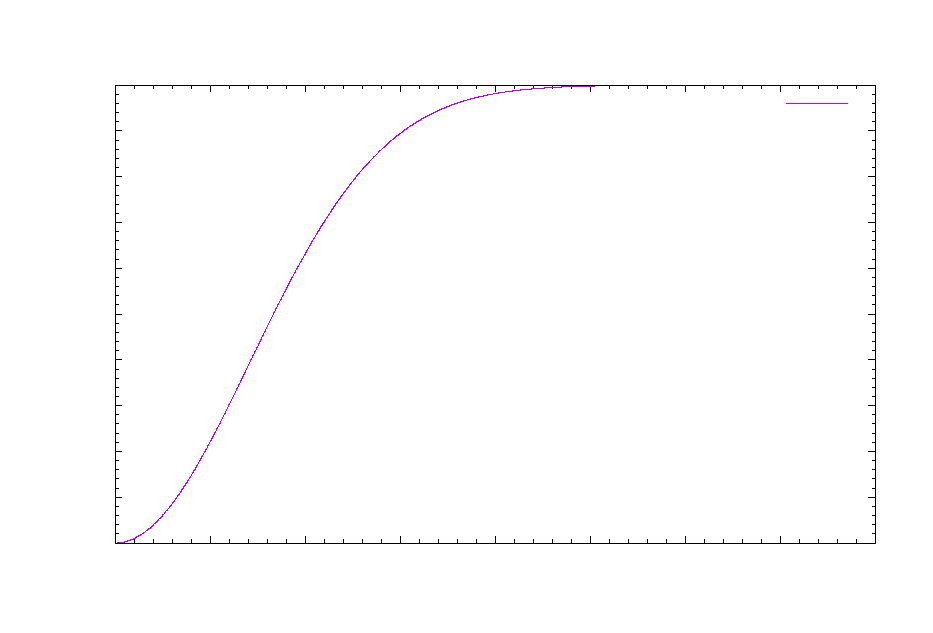
\includegraphics[width={432.00bp},height={288.00bp}]{leistung}}%
    \gplfronttext
  \end{picture}%
\endgroup

			\caption{\centering Intensitätsprofil eines Laserstrahls}
			\label{fig:tvfour-leistung}
			\vspace{-1em}
		\end{figure}
		Nun plotten wir die Daten aus dem Versuch und führe eine Kurveanpassung mit:
		\begin{align}
			P(d) &= A\omega^2\left(1 - \exp{-2\left(\frac{d}{2\omega}\right)^2}\right) = A\omega^2\left(1 - \exp{-\frac{d^2}{2\omega^2}}\right) \\
			&= AW\left(1 - \exp{-\frac{d^2}{2W}}\right)
		\end{align}
		Bei der Kurvenanpassung wird einen Fehler $\Delta P$ von \SI{0.1}{\milli\watt} und einen Fehler $\Delta d$ von \SI{0.1}{\milli\meter} angenommen.

		Aus \gnuplot{} (Appendix \ref{appdx:gnuplottv4}) erhalten wir:
		\begin{figure}[H]
			\centering
			% GNUPLOT: LaTeX picture with Postscript
\begingroup
  \makeatletter
  \providecommand\color[2][]{%
    \GenericError{(gnuplot) \space\space\space\@spaces}{%
      Package color not loaded in conjunction with
      terminal option `colourtext'%
    }{See the gnuplot documentation for explanation.%
    }{Either use 'blacktext' in gnuplot or load the package
      color.sty in LaTeX.}%
    \renewcommand\color[2][]{}%
  }%
  \providecommand\includegraphics[2][]{%
    \GenericError{(gnuplot) \space\space\space\@spaces}{%
      Package graphicx or graphics not loaded%
    }{See the gnuplot documentation for explanation.%
    }{The gnuplot epslatex terminal needs graphicx.sty or graphics.sty.}%
    \renewcommand\includegraphics[2][]{}%
  }%
  \providecommand\rotatebox[2]{#2}%
  \@ifundefined{ifGPcolor}{%
    \newif\ifGPcolor
    \GPcolortrue
  }{}%
  \@ifundefined{ifGPblacktext}{%
    \newif\ifGPblacktext
    \GPblacktexttrue
  }{}%
  % define a \g@addto@macro without @ in the name:
  \let\gplgaddtomacro\g@addto@macro
  % define empty templates for all commands taking text:
  \gdef\gplbacktext{}%
  \gdef\gplfronttext{}%
  \makeatother
  \ifGPblacktext
    % no textcolor at all
    \def\colorrgb#1{}%
    \def\colorgray#1{}%
  \else
    % gray or color?
    \ifGPcolor
      \def\colorrgb#1{\color[rgb]{#1}}%
      \def\colorgray#1{\color[gray]{#1}}%
      \expandafter\def\csname LTw\endcsname{\color{white}}%
      \expandafter\def\csname LTb\endcsname{\color{black}}%
      \expandafter\def\csname LTa\endcsname{\color{black}}%
      \expandafter\def\csname LT0\endcsname{\color[rgb]{1,0,0}}%
      \expandafter\def\csname LT1\endcsname{\color[rgb]{0,1,0}}%
      \expandafter\def\csname LT2\endcsname{\color[rgb]{0,0,1}}%
      \expandafter\def\csname LT3\endcsname{\color[rgb]{1,0,1}}%
      \expandafter\def\csname LT4\endcsname{\color[rgb]{0,1,1}}%
      \expandafter\def\csname LT5\endcsname{\color[rgb]{1,1,0}}%
      \expandafter\def\csname LT6\endcsname{\color[rgb]{0,0,0}}%
      \expandafter\def\csname LT7\endcsname{\color[rgb]{1,0.3,0}}%
      \expandafter\def\csname LT8\endcsname{\color[rgb]{0.5,0.5,0.5}}%
    \else
      % gray
      \def\colorrgb#1{\color{black}}%
      \def\colorgray#1{\color[gray]{#1}}%
      \expandafter\def\csname LTw\endcsname{\color{white}}%
      \expandafter\def\csname LTb\endcsname{\color{black}}%
      \expandafter\def\csname LTa\endcsname{\color{black}}%
      \expandafter\def\csname LT0\endcsname{\color{black}}%
      \expandafter\def\csname LT1\endcsname{\color{black}}%
      \expandafter\def\csname LT2\endcsname{\color{black}}%
      \expandafter\def\csname LT3\endcsname{\color{black}}%
      \expandafter\def\csname LT4\endcsname{\color{black}}%
      \expandafter\def\csname LT5\endcsname{\color{black}}%
      \expandafter\def\csname LT6\endcsname{\color{black}}%
      \expandafter\def\csname LT7\endcsname{\color{black}}%
      \expandafter\def\csname LT8\endcsname{\color{black}}%
    \fi
  \fi
    \setlength{\unitlength}{0.0500bp}%
    \ifx\gptboxheight\undefined%
      \newlength{\gptboxheight}%
      \newlength{\gptboxwidth}%
      \newsavebox{\gptboxtext}%
    \fi%
    \setlength{\fboxrule}{0.5pt}%
    \setlength{\fboxsep}{1pt}%
\begin{picture}(8640.00,5760.00)%
    \gplgaddtomacro\gplbacktext{%
      \csname LTb\endcsname%%
      \put(550,704){\makebox(0,0)[r]{\strut{}$0$}}%
      \put(550,1192){\makebox(0,0)[r]{\strut{}$1$}}%
      \put(550,1681){\makebox(0,0)[r]{\strut{}$2$}}%
      \put(550,2169){\makebox(0,0)[r]{\strut{}$3$}}%
      \put(550,2657){\makebox(0,0)[r]{\strut{}$4$}}%
      \put(550,3146){\makebox(0,0)[r]{\strut{}$5$}}%
      \put(550,3634){\makebox(0,0)[r]{\strut{}$6$}}%
      \put(550,4122){\makebox(0,0)[r]{\strut{}$7$}}%
      \put(550,4611){\makebox(0,0)[r]{\strut{}$8$}}%
      \put(550,5099){\makebox(0,0)[r]{\strut{}$9$}}%
      \put(682,484){\makebox(0,0){\strut{}$0$}}%
      \put(1627,484){\makebox(0,0){\strut{}$2$}}%
      \put(2572,484){\makebox(0,0){\strut{}$4$}}%
      \put(3517,484){\makebox(0,0){\strut{}$6$}}%
      \put(4463,484){\makebox(0,0){\strut{}$8$}}%
      \put(5408,484){\makebox(0,0){\strut{}$10$}}%
      \put(6353,484){\makebox(0,0){\strut{}$12$}}%
      \put(7298,484){\makebox(0,0){\strut{}$14$}}%
      \put(8243,484){\makebox(0,0){\strut{}$16$}}%
    }%
    \gplgaddtomacro\gplfronttext{%
      \csname LTb\endcsname%%
      \put(209,2901){\rotatebox{-270}{\makebox(0,0){\strut{}Transmittierte Leistung $P$ ($\si{\milli\watt}$)}}}%
      \put(4462,154){\makebox(0,0){\strut{}Durchmesser $d$ ($\si{\milli\meter}$)}}%
      \csname LTb\endcsname%%
      \put(7256,1427){\makebox(0,0)[r]{\strut{}$1,05673\cdot7,45305\left(1 - \exp{-\frac{d^2}{2(7,45305)}}\right)$}}%
      \csname LTb\endcsname%%
      \put(7256,987){\makebox(0,0)[r]{\strut{}Messpunkte}}%
      \csname LTb\endcsname%%
      \put(4462,5429){\makebox(0,0){\strut{}Transmittierte Leistung gegen Strahldurchmesser}}%
    }%
    \gplbacktext
    \put(0,0){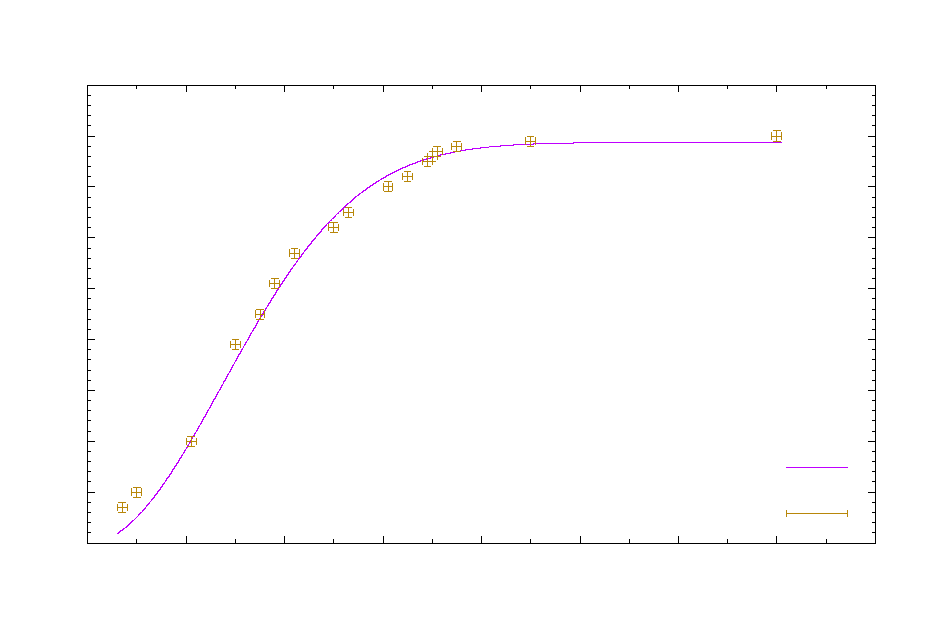
\includegraphics[width={432.00bp},height={288.00bp}]{tv4-plot}}%
    \gplfronttext
  \end{picture}%
\endgroup

			\caption{\centering Intensitätsprofil des grünen Lasers $(\chi^2_{\text{red}} = 1,77774 \approx 1 \Rightarrow \text{Gute Anpassung})$ }
			\label{fig:tvfour-leistung}
			\vspace{-1em}
		\end{figure}
		mit dem Endergebnis:
		\begin{equation*}
			\begin{tabu}{lll}
				\toprule
				\text{Variable} & \text{Wert} & \text{Gerundet} \\
				\midrule
				A        & \SI{1.0567(488)}{\milli\watt\per\meter\squared} & \SI{1.06(5)}{\milli\watt\per\meter\squared}\\
				\omega^2 & \SI{7.4531(4013)}{\milli\meter\squared}         & \SI{7.5(5)}{\milli\meter\squared} \\
				\bottomrule
			\end{tabu}
		\end{equation*}
		Da die Kurveanpassung ziemlich gut war, können wir daraus schließen, dass die experimentelle Werte die theoretische Gleichung wirklich übereinstimmt. Es ist auch zu bemerken, dass die erhaltenen Kurve komplementär zum gaußförmigen Intensitätsprofil des Laserstrahls ist.
	\subsection{Divergenzwinkel}
		Der Halbdivergenzwinkel haben wir als $\varphi = \SI{3}{\degree}$ im Versuch bestimmt. Mit einer Bestrahlungsdauer von $\SI{150}{\second}$ liegen die Bestrahlung immer noch im Bereich $\SI{e2}{\second}$ bis $\SI{3e4}{\second}$ und wir haben als MZB für den grünen Laser $\text{MZB} = \SI{10}{\watt\per\meter\squared}$.

		Wir nehmen noch zusätzlich an, dass der Fokus eine Durchmesser von $d = \SI{1}{\milli\meter}$ hat.

		Somit erhalten wir mit $P = \SI{8.4}{\milli\watt}$ als $r_{\text{NOHD}}$:
		\begin{align}
			r_{\text{NOHD}} &= \frac{1}{\theta} \times \frac{180}{\pi}\left(\sqrt{\frac{8P}{\pi\text{MZB}}} - d\right) \notag\\
			&= \frac{1}{2\varphi} \times \frac{180}{\pi}\left(\sqrt{\frac{8P}{\pi\text{MZB}}} - d\right) \notag\\
			&= \frac{1}{2(3)} \times \frac{180}{\pi}\left(\sqrt{\frac{8(\SI{8.4e-3}{\watt})}{\pi(\SI{10}{\watt\per\meter\squared})}} - \SI{1e-3}{\meter}\right) \notag \\
			&= \SI{0.43}{\meter} = \SI{43}{\centi\meter}
		\end{align}
		Wir haben während des Versuchs die Divergenzwinkel bei einem Abstand größer als \SI{43}{\centi\meter} gemessen, somit ist man bei diesem Abstand am Ende des Tischs schon vom Laser sicher. 
	\nonum



